%\documentclass[12pt,fleqn]{report}
%\marginsize{left}{right}{top}{bottom}
\documentclass[10pt,fleqn,a4paper]{report}
\usepackage{anysize}
\marginsize{2cm}{2cm}{2cm}{2cm}
\usepackage{color}
\usepackage{multicol}
\usepackage{makeidx}
\usepackage{bm}
\usepackage[normalem]{ulem}
\makeindex

\usepackage[linkbordercolor={0 0 1}]{hyperref}
\usepackage[pdftex]{graphicx}

\definecolor{light-gray}{gray}{0.95}

\newcommand{\keyword}[1]{\index{Keywords!{\tt #1}} {\tt #1}}
\newcommand{\cv}[1]{\index{Collective variables!{#1}}
\index{{#1}|see{Collective variables, {#1}}} }
\newcommand{\plumed}{{\tt PLUMED}}


\newcommand{\esempio}[1]{
\vspace{10pt}
\begin{flushright}
\colorbox{light-gray}{
   \begin{minipage}{13cm}
       \scriptsize{
{\fontfamily{phv} \fontseries{b}
 \selectfont Example. \\
 \fontseries{m} \selectfont #1 } }
\end{minipage}}
\end{flushright}
\vspace{20pt}
}

\begin{document}

%% -----------------------------------------------------------------------------------------
\begin{titlepage}
\vspace{4cm}
\begin{flushleft}
{
 { \fontencoding{OT1}\fontfamily{phv} \fontshape{i} \fontseries{b} \Large{a micro  PLUMED2.0 Tutorial for ESPResSo users}} \\ \vspace{.5cm}
 { \fontencoding{OT1}\fontfamily{phv} \fontshape{sl} \selectfont \Large{PLUMED2.0: \\ portable plugin for free-energy calculations \\ with  molecular dynamics}}
}
\rule{12cm}{4pt}
\end{flushleft}
\vspace{1cm}
\begin{figure}[here!]
\begin{center}

\includegraphics[width=15cm,angle=0]{./figures/logo}
\end{center}
\end{figure}
\vspace{1cm}
\begin{flushright}
 \fontencoding{OT1}\fontfamily{phv} \fontseries{b} \fontshape{i} \large{
 ESPResSo summer school 2013
 } \\ 
 \vspace{1cm}

 \fontencoding{OT1}\fontfamily{phv} \fontseries{b} \fontshape{i} \large{Organized by CECAM, SimTech, ICP and University of Stuttgart} \\
\vspace{1cm}
 
 \fontencoding{OT1}\fontfamily{phv} \fontseries{b} \fontshape{i} \large{Institute for Computational Physics, Stuttgart University, Germany} \\
 \fontencoding{OT1}\fontfamily{phv} \fontseries{b} \fontshape{i} \large{October 7 - October 11, 2013}
\end{flushright}
%% -----------------------------------------------------------------------------------------



\end{titlepage}

\newpage

\noindent
\Large{This document and the relative computer exercises have been written by Davide Branduardi and is based on a previous tutorial held in CECAM, Lausanne in 2010 whose authors are:}\\ \\
\Large{Massimiliano Bonomi\\ Davide Branduardi\\ Giovanni Bussi\\ 
Francesco Gervasio\\ Alessandro Laio\\ Fabio Pietrucci}\\ \\ \\ \\
\large{
Tutorial website:\\
{\tt http://sites.google.com/site/plumedtutorial2010/}\\ \\ 
PLUMED website:\\
{\tt http://www.plumed-code.org}\\ \\ 
PLUMED users Google group:\\
{\tt plumed-users@googlegroups.com}\\ \\
PLUMED reference articles: \\ \\
M.~Bonomi, D.~Branduardi, G.~Bussi, C.~Camilloni, D.~Provasi, P.~Raiteri,
D.~Donadio, F.~Marinelli, F.~Pietrucci, R.A.~Broglia and M.~Parrinello,
\href{http://dx.doi.org/10.1016/j.cpc.2009.05.011}{},
 Comp.~Phys.~Comm. 2009 vol. 180 (10) pp. 1961-1972. \\ \\
 G.A.~Tribello, M.~Bonomi, D.~Branduardi, C.~Camilloni, G.~Bussi
 \href{http://dx.doi.org/10.1016/j.cpc.2013.09.018}{},
  Comp.~Phys.~Comm. 2013 in press. \\
}


%\newpage
\clearpage

\tableofcontents

\chapter{What PLUMED is and what it can do}
PLUMED is a library  released under L-GPL license  interfaced to a number of molecular dynamics engines (beyond ESPResSo: NAMD, GROMACS, LAMMPS and quantum Espresso) that enables the code to perform a number of different kinds of \uline{enhanced sampling calculations}. 
Its core consists in a routine that takes the position of the atoms at each time-step of the molecular dynamics and \uline{introduces forces according to the specific configuration of the system}: this is the core of many enhanced sampling calculations. Since this is a very tiny link to the MD code, this can be done in a rather general way and that is on of the main reasons why many MD codes incorporates it. In general, PLUMED can also do something simpler like calculating strange observable that you might be interested along the run and print them for you. Since the tcl capabilities of ESPResSo are quite remarkable, we will not spend much time on this.

The addition of such special forces allow for two things: let you build a free energy landscape of your system, projected on the descriptors of your choice associated to conformational transitions,  chemical reaction or phase transitions and also accelerates the dynamics of your system which is particularly important when dealing with activated events.

In general, the free energy of a system in a specific point of the phase space can be defined as

\begin{equation}
F({\bf s})=-\frac{1}{\beta}\log P({\bf s})
\end{equation}
where $F$ is the Helmoltz's free energy, $s$ is a descriptor of the system (a bond distance, angle, or another generic order parameter of some sort), 
$P({\bf s})$ is the probability that the system is in the state labelled by the descriptor ${\bf s}$ (here, for the sake of generality reported in bold since it can be defined in many dimensions), $\beta=1/k_BT$ where $k_B$ is the Boltzmann constant and $T$ is the temperature of the system.

Therefore, based on the ergodic hypothesis, just building an histogram of the conformations along your molecular dynamics run is the easiest way one can build a free-energy profile as a function of some parameter.

Unfortunately, very often it happens that the exploration via MD is all but exhaustive. In fact the system may stay trapped in some minimum inasmuch the kinetic energy provided from the thermostat (which is $0.5 k_BT$ = 0.3 kcal/mol per degree of freedom at 300 K) very often does not allow for the the overcoming of barriers within the usual time span of a MD simulations (typically tens to hundreds of ps for ab initio MD, up to several $\mu$s for classical-force-field-based MD). In this case we say that the system is in a "metastable state" which is  exemplified in the Fig. \ref{partial_conv}

\begin{figure}[h!]
\begin{center}
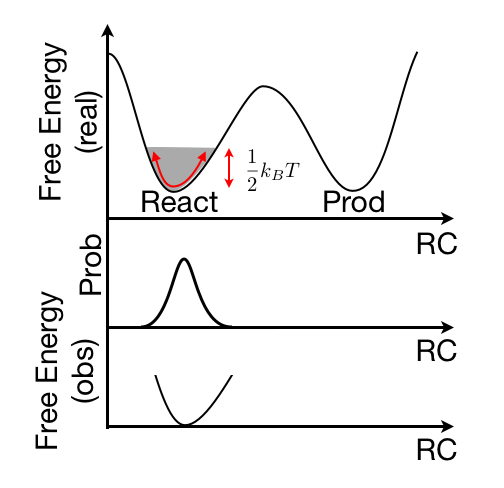
\includegraphics[width=14cm,angle=0]{./figures/partial_conv}
\caption{A sketch of the effect of partial sampling during MD. A basin that is there is not sampled just because it takes too much time to cross the barrier.}
\label{part_conv}
\end{center}
\end{figure} 

In order to illustrate this, let us consider a typical barrier for a chemical reaction: $\Delta U^\ddagger\simeq8$ kcal/mol. One can estimate the rate of a reaction by using the Arrhenius equation that reads
\begin{equation}
\nu(T)=\nu_0\exp^{-\frac{\Delta U^\ddagger}{k_BT} }.
\end{equation}
By considering $\nu_0$ for a typical covalent bond, $\nu_0 \rm =5\ 10^9 s^{-1}$, as an upper bound, one easily get a rate of $\rm 7\ 10^3 $ events per second. Therefore, each single event can well take up to a millisecond and the observation of one single event is (very) fortuitous in the typical timescales of a even classical MD. Moreover, since the estimate of the probability requires converged statistics, the converged free-energy calculation can require even much more time. 
Therefore, either you find smart ways of sampling the phase space or you should find some workaround for this. PLUMED implements some "force-based" workaround to this aim.
%



\chapter{Basics: how to enable PLUMED2.0 in ESPResSo}

Enabling PLUMED within ESPResSo requires you to install various packages.
\begin{itemize} 
\item You need to download the version of ESPResSo that you find at 
\url{http://davidebr.github.io/espresso/}. 
\item You need a version of PLUMED2.0. The stable version can be found at 
\url{http://www.plumed-code.org/} while a bleeding-edge version can be found on
\url{https://github.com/plumed/plumed2}.
\item You need BLAS and LAPACK libraries installed. These are generally available on most systems
\item (optional) a version of libmateval \url{http://www.gnu.org/software/libmatheval/} which allows to invent crazy variables of your choice. If you are a beginner you might be happy with what is already provided within PLUMED2.0.
\end{itemize}

\subsection{Compiling PLUMED2.0}
I recommend to compile plumed with an MPI compiler. Gcc is perfect for this.
Information on PLUMED2.0 are at \url{http://plumed.github.io/doc-v2.0/user-doc/html/index.html} and the installation details are reported in a link on that page. 
Supposing that your PLUMED2.0 version is downloaded in
\begin{verbatim}
/my/path/to/plumed2
\end{verbatim}
you should source the file contained in it
\begin{verbatim}
source /my/path/to/plumed2/sourceme.sh
\end{verbatim}
This allows all the environment variables that you need to be properly set.
Then you proceed in compiling plumed as reported.

\subsection{Compiling ESPResSo}
You can proceed in the usual way with ESPResSo but you should define two flags before configuring
\begin{verbatim}
export CPPFLAGS=" -I /my/path/to/plumed2/src/wrapper "
export LDFLAGS=" -L /my/path/to/plumed2/src/lib -lplumed "
export LD_LIBRARY_PATH=${LD_LIBRARY_PATH}:/my/path/to/plumed2/src/lib/
\end{verbatim}
and then you proceed with bootstrapping, configuring and making.

At this point your ESPResSo is ready to go!

Note: it is possible that this version will not be regularly updated.
In general you can update yourself just by merging the master on the current branch. 
This requires a bit of git expertise though. 

\subsection{A note regarding the specific location in which is performed the tutorial}

In the tutorial room there are a number of available PCs. They are numbered from cip1 to cip24.

Before running the PLUMED2.0 version of ESPResSo you should set up the environment like this
\begin{verbatim}
export LD_LIBRARY_PATH=
   /home/davide/software/plumed2/src/lib:$LD_LIBRARY_PATH
export LD_LIBRARY_PATH=
   /home/davide/software/libmatheval-1.1.10_install/lib64:$LD_LIBRARY_PATH
 source  /home/davide/software/plumed2/sourceme.sh 
\end{verbatim}

Now you can use the executable of ESPResSo I compiled for you from 
\begin{verbatim}
/home/davide/software/espresso/Espresso
\end{verbatim}
and you can link it or copy as you wish.

{\bf For your convenience I made all those steps in a single bash file to source}
\begin{verbatim}
source /home/davide/software/espresso/SETUP_FULL_ENVIRONMENT.sh
\end{verbatim}

You should also have PLUMED2.0 as command line tool.
Just try
\begin{verbatim}
plumed help
\end{verbatim}
and you should have a list of options.

In the directory
\begin{verbatim}
/home/davide/software/espresso/plumed_tests
\end{verbatim}

you have the exercises. Copy them in your local directory.

\subsection{Switching on PLUMED2.0}
Now, if you do not explicitly ask for PLUMED2.0, your code will work normally as it was without it.
If you want to enable it you should include a line in your tcl script that you use as input in ESPResSo.
\begin{verbatim}
setmd plumedison 1
\end{verbatim}
At this point your code expects a file named \texttt{plumed.dat}. 
This is important because plumed get its command from an external file and not from the tcl interface. The tcl interface is only used to switch plumed on and off and to define the input file.
If you do not have the input file, plumed
will crash but at least you will see it alive and kicking. 
Alternatively you can simply make 
\begin{verbatim}
touch plumed.dat
\end{verbatim}
and your calculation will proceed normally, without doing anything but producing since plumed 
is not instructed to do anything. You should get 
the plumed banner as soon as you use the \texttt{integrate} command.

%You can define your input file by using in the tcl input, for example 
%\begin{verbatim}
%setmd plumedison 1
%set plumed_input [open "myplumed.dat" "w"]
%puts  $plumed_input "d1: DISTANCE ATOMS=1,2"
%puts  $plumed_input "PRINT ARG=* STRIDE=50 FILE=COLVAR"
%close $plumed_input
%setmd plumedfile myplumed.dat
%\end{verbatim}

So far so good, now let's see what you can do with it!

\chapter{Basics: calculate a distance between two atoms}

For the sake of discussion, the examples that will follow are generated just by hacking 
the example in \texttt{samples/tutorial.tcl} that you find in the normal ESPResSo distribution.
A sketch of it is in Fig. \ref{system}. It is a small 40-mer in a set of other particles.

\begin{figure}[h!]
\begin{center}
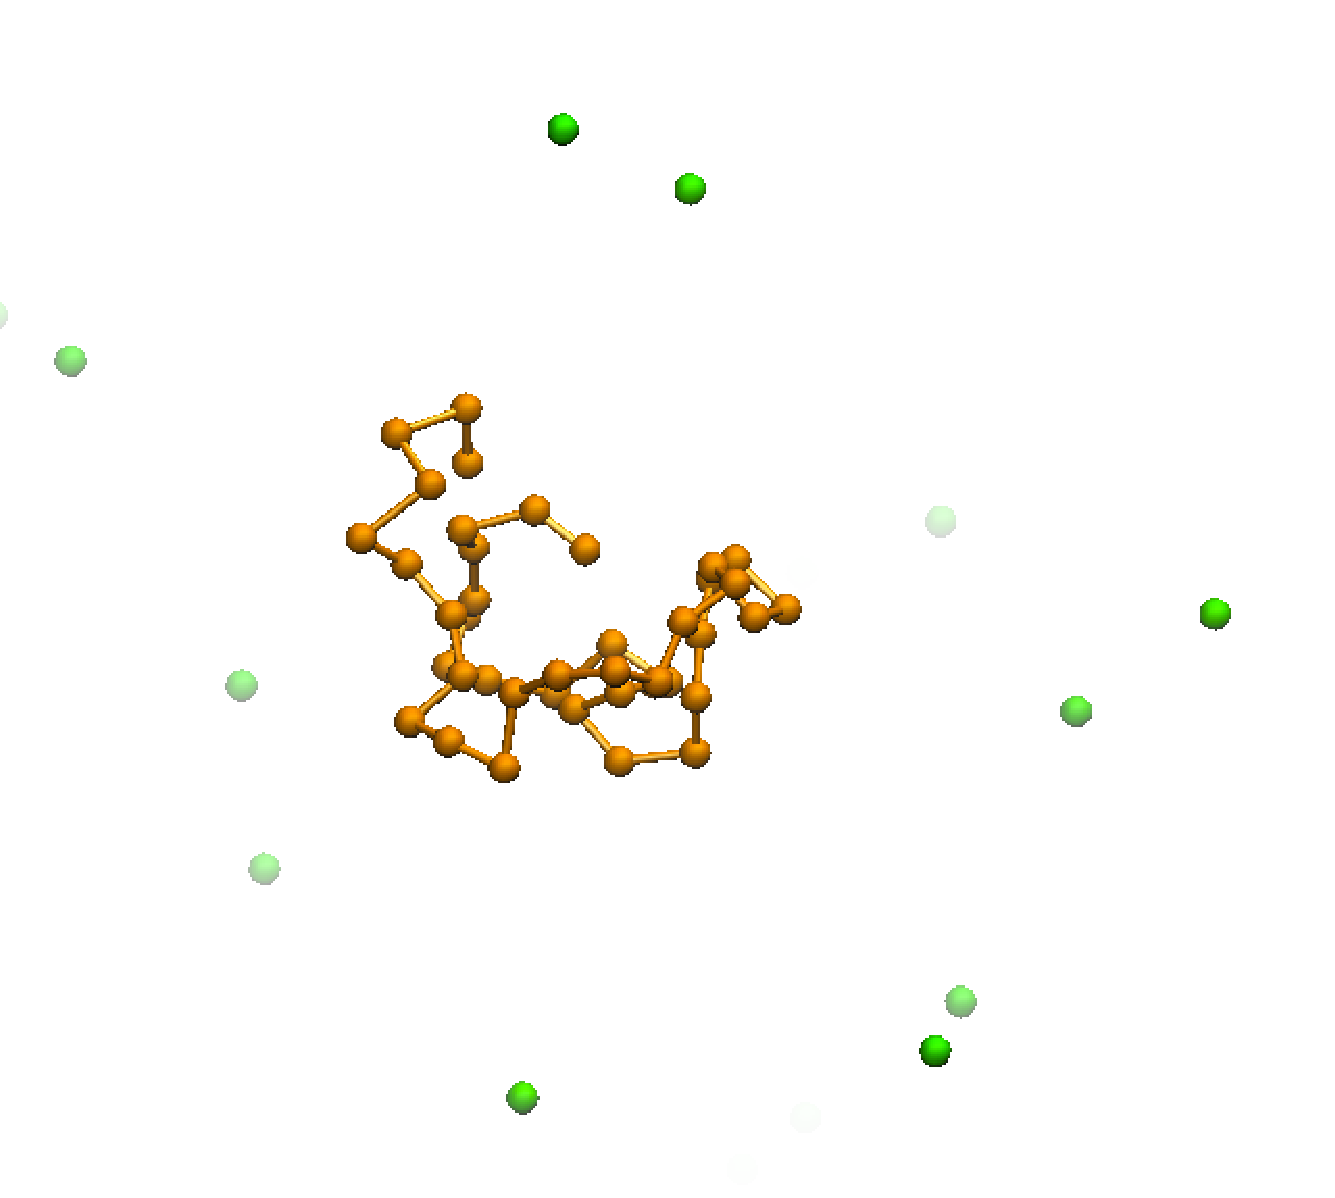
\includegraphics[width=14cm,angle=0]{./figures/system}
\caption{The toy system used in the examples.}
\label{system}
\end{center}
\end{figure} 

As first example we run something which is similar to the example previously reported.
So you have to add the following lines to the \texttt{tutorial.tcl} (already provided in the example)
\begin{verbatim}
setmd plumedison 1
setmd plumedfile plumedinput.dat
\end{verbatim}
which switch on plumed and determine the name of plumed input.
Additionally you have to
create a the plumed input file \texttt{plumedinput.dat} which contains the following lines
\begin{verbatim}
# (hashes are comments)
# a descriptor labeled "d1": is the distance between the atom 1 and the atom 40
# (numbering starts with 0)
d1:  DISTANCE ATOMS=1,40
# print all the previous actions (in this case only the distance)
# every 50 time steps on a file called COLVAR
PRINT ARG=* STRIDE=50 FILE=COLVAR
\end{verbatim}
which trivially calculates the distance between the two end of the chain and print it out on a file named \texttt{COLVAR}.
In the tutorial location you can run the example like this
\begin{verbatim}
/home/davide/software/espresso/Espresso tutorial.tcl
\end{verbatim}

As soon as the first \texttt{integrate} command is run you get a banner like this
\begin{verbatim}
PLUMED IS ON AND INSTALLED
PLUMEDFILE IS plumed.dat
.....(something here)
PLUMED: Molecular dynamics engine: espresso
PLUMED: Precision of reals: 8
PLUMED: Running over 1 node
PLUMED: Number of atoms: 80
PLUMED: File suffix:
PLUMED: FILE: plumed.dat
PLUMED: Action DISTANCE
PLUMED:   with label d1
PLUMED:   between atoms 1 40
PLUMED:   using periodic boundary conditions
PLUMED: Action PRINT
PLUMED:   with label @1
PLUMED:   with stride 50
PLUMED:   with arguments d1
PLUMED:   on file COLVAR
PLUMED:   with format  \%f
PLUMED: END FILE: plumed.dat
PLUMED: Timestep: 0.010000
...(something else here)
\end{verbatim}
The first two lines are printed from ESPResSo code and just say that the installation was ok. 
The following will help you to understand wether plumed got your input right.
You can see that two "Actions" are created, one for each line of the input. Note that we gave a label to one action (DISTANCE) but not to the second. Plumed is giving some default name:  \texttt{@1} in this case.

When running the example provided you get an output file called \texttt{COLVAR} that contains the time and all the actions (i.e. the distance value along time):
\begin{verbatim}
#! FIELDS time d1
 0.500000 2.374363
 1.000000 2.551184
 1.500000 2.392192
 2.000000 2.292906
 2.500000 2.789281
 3.000000 2.782809
 ....
\end{verbatim}
This, by itself can be used to create some histogram to produce a free energy.

Note that many descriptors can be used simultaneously and 
the full list of available descriptors can be found at \url{http://plumed.github.io/doc-v2.0/user-doc/html/index.html}.

\vspace{1cm}
There is also an additional flag you can use in the ESPResSo input.
\begin{verbatim}
setmd plumedreset 1
\end{verbatim}
This makes so that plumed forgets the previous history at every \texttt{integrate} command. This means that all the biases and other history-dependent variables are forgot and a new \texttt{COLVAR} file is produced. Note that the previous files are, by default, renamed into \texttt{bak.0.COLVAR,  bak.1.COLVAR, ... }

 This can be useful if, in the same tcl file you restart your system several time since you can reinitialize plumed every time and eve distinct output files. 

\chapter{Biasing the system: steered MD}
In order to show how you can bias your system we will start from the previous example and extend the input:
\begin{verbatim}
# the distance we have seen before
d1: DISTANCE ATOMS=1,40
# add a moving restraint using d1
# stretching from 2 to 40 at 20000 time step and then 
# stretching back at 2
MOVINGRESTRAINT ...
  ARG=d1
  STEP0=0          AT0=2.0    KAPPA0=5.0
  STEP1=20000  AT1=40.0  KAPPA1=5.0
  STEP2=40000  AT2=2.0    KAPPA2=5.0
... MOVINGRESTRAINT
# the print everything
PRINT ARG=* STRIDE=50 FILE=COLVAR
# this prints only the center of the harmonic potential and 
# the work (see later)
PRINT ARG=@1.d1_cntr,@1.d1_work STRIDE=50 FILE=WORK
\end{verbatim}
This, as evident, intruduce a moving restraint on the distance which amount to introduce a moving harmonic force on the distance that augment the hamiltonian of the system $H({\bf x})$
\begin{equation}
H'({\bf x},t)=H({\bf x})+\frac{k}{2}\left(\bf{s}({\bf x}\right) - x_0 -v t)^2
\end{equation}
where $\bf{s} \left( {\bf x} \right)$ is in this case the distance calculated and where the velocity of the center of the harmonic potential is given by
\begin{equation}
v= (\texttt{AT1}-\texttt{AT0})/(\texttt{STEP1-STEP0})
\end{equation}
The output from the banner is a little more complex
\begin{verbatim}
PLUMED: Action DISTANCE
PLUMED:   with label d1
PLUMED:   between atoms 1 40
PLUMED:   using periodic boundary conditions
PLUMED: Action MOVINGRESTRAINT
PLUMED:   with label @1
PLUMED:   with stride 1
PLUMED:   with arguments d1
PLUMED:   step0 0
PLUMED:   at 2.000000
PLUMED:   with force constant 5.000000
PLUMED:   step1 20000
PLUMED:   at 40.000000
PLUMED:   with force constant 5.000000
PLUMED:   step2 40000
PLUMED:   at 2.000000
PLUMED:   with force constant 5.000000
PLUMED:   added component to this action:  @1.bias
PLUMED:   added component to this action:  @1.force2
PLUMED:   added component to this action:  @1.d1_cntr
PLUMED:   added component to this action:  @1.d1_work
PLUMED:   Bibliography [2]
PLUMED: Action PRINT
PLUMED:   with label @2
PLUMED:   with stride 50
PLUMED:   with arguments d1 @1.bias @1.force2 @1.d1_cntr @1.d1_work
PLUMED:   on file COLVAR
PLUMED:   with format  \%f
PLUMED: END FILE: plumed.dat
\end{verbatim}
which is worth having a look at since one can see new interesting stuff.
For example the action \texttt{MOVINGRESTRAINT} creates four different components, namely the bias, the force, the position of the center of the harmonic potential and the work which is obtained via
\begin{eqnarray}
W=\int_0^{t_s}dt\ \frac{\partial H'({\bf x},t)}{\partial t}
\end{eqnarray}
and this is a very rough estimate of the free energy difference between the two states. 
For something more accurate one should employ Jarzynski or Crooks equality.

The \texttt{COLVAR} file thus obtained looks like
\begin{verbatim}
#! FIELDS time d1 @1.bias @1.force2 @1.d1_cntr @1.d1_work
 0.500000 2.367756 0.185989 1.859890 2.095000 -0.016664
 1.000000 2.318884 0.041528 0.415279 2.190000 -0.128000
 1.500000 2.553767 0.180589 1.805890 2.285000 -0.181267
 2.000000 2.828038 0.501846 5.018459 2.380000 -0.352905
....
\end{verbatim}
in which all the fields declared are reported.
On the other side the file named \texttt{WORK} will contain only the requested features 
(besides time, which always appear)
\begin{verbatim}
#! FIELDS time @1.d1_cntr @1.d1_work
 0.500000 2.095000 -0.016664
 1.000000 2.190000 -0.128000
 1.500000 2.285000 -0.181267
\end{verbatim}
It is funny to plot this work as a function of time (see Fig. \ref{work})
\begin{figure}[h!]
\begin{center}
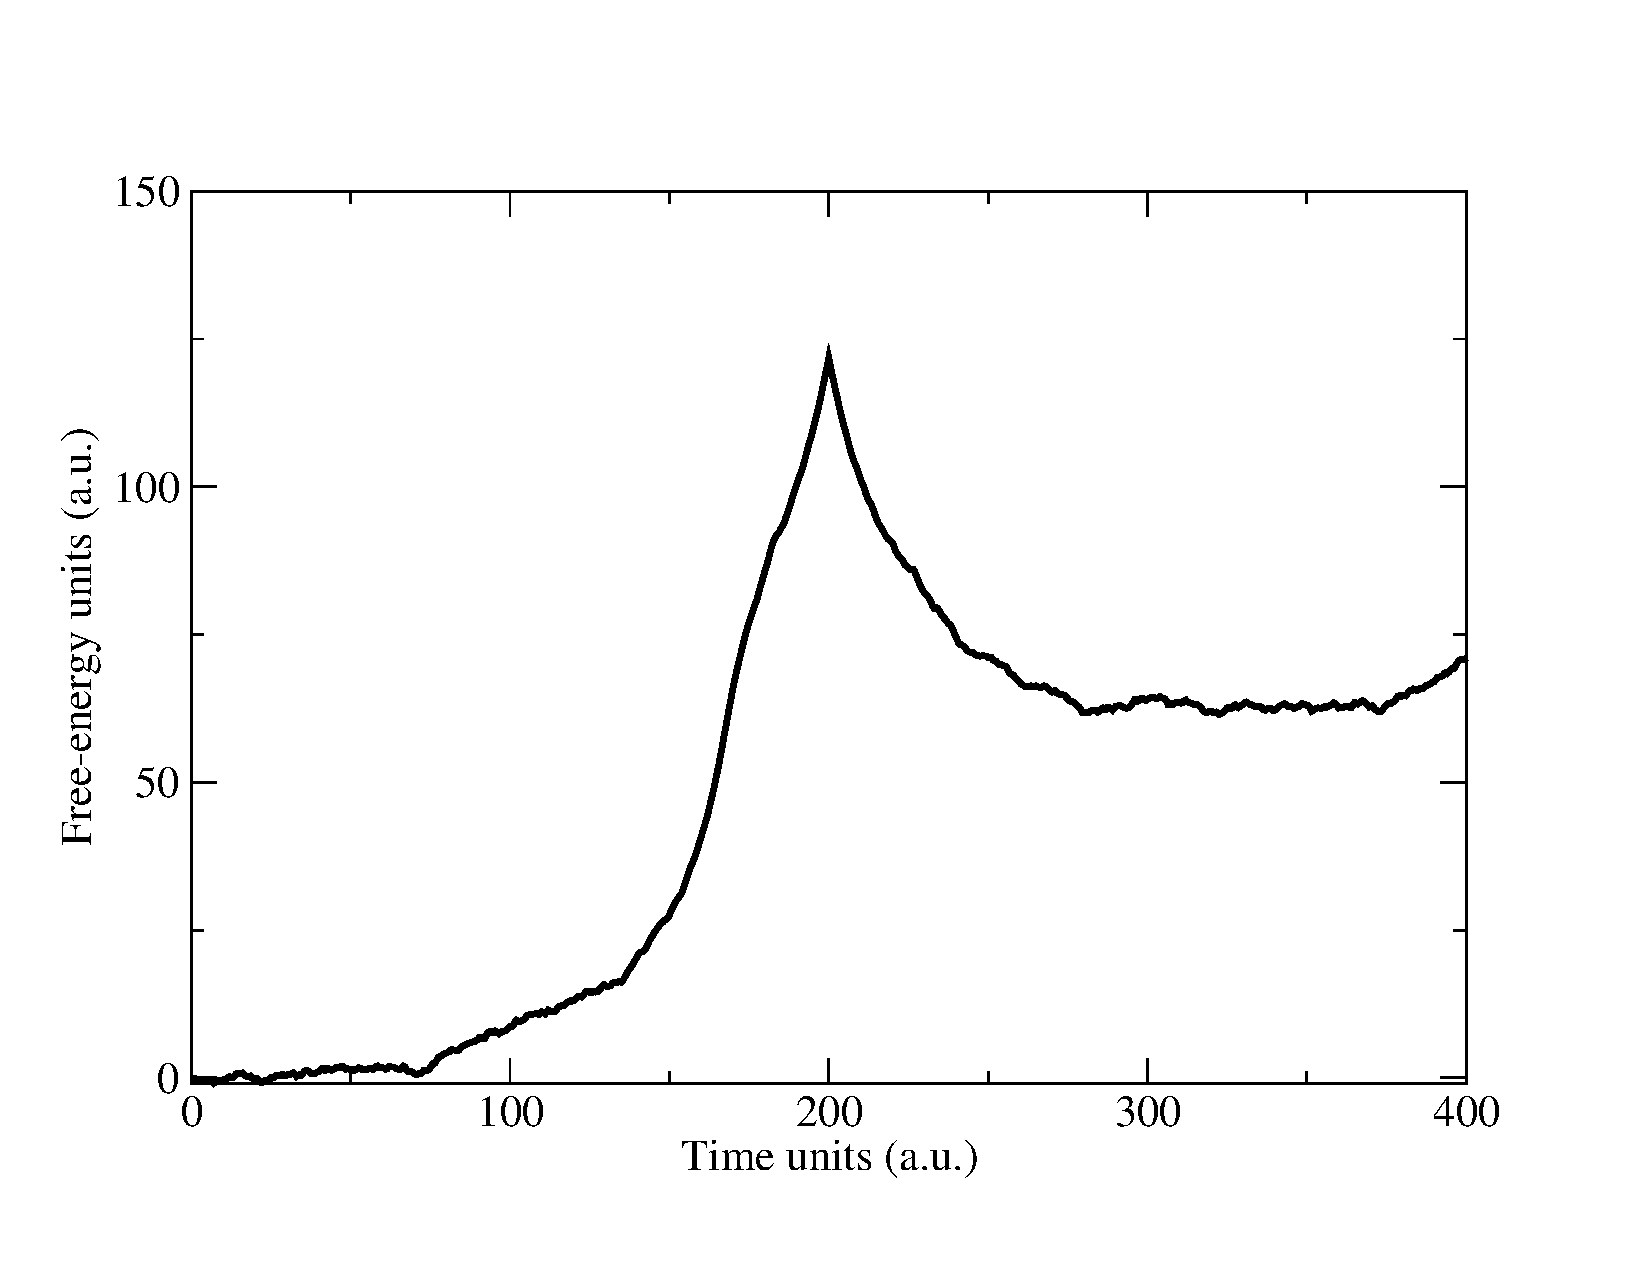
\includegraphics[width=14cm,angle=0]{./figures/work}
\caption{Work profile during the pulling forward and backward}
\label{work}
\end{center}
\end{figure} 
that gives you the idea that when you pull forward you do not get the same work as you are going backward. By averging on a lot of profiles then you get a free energy.

In practice you can do this in \texttt{gnuplot}. After having invoked it, you can use the following commands
\begin{verbatim}
gnuplot> plot "WORK" u 1:3
\end{verbatim}


\begin{figure}[h!]
\begin{center}
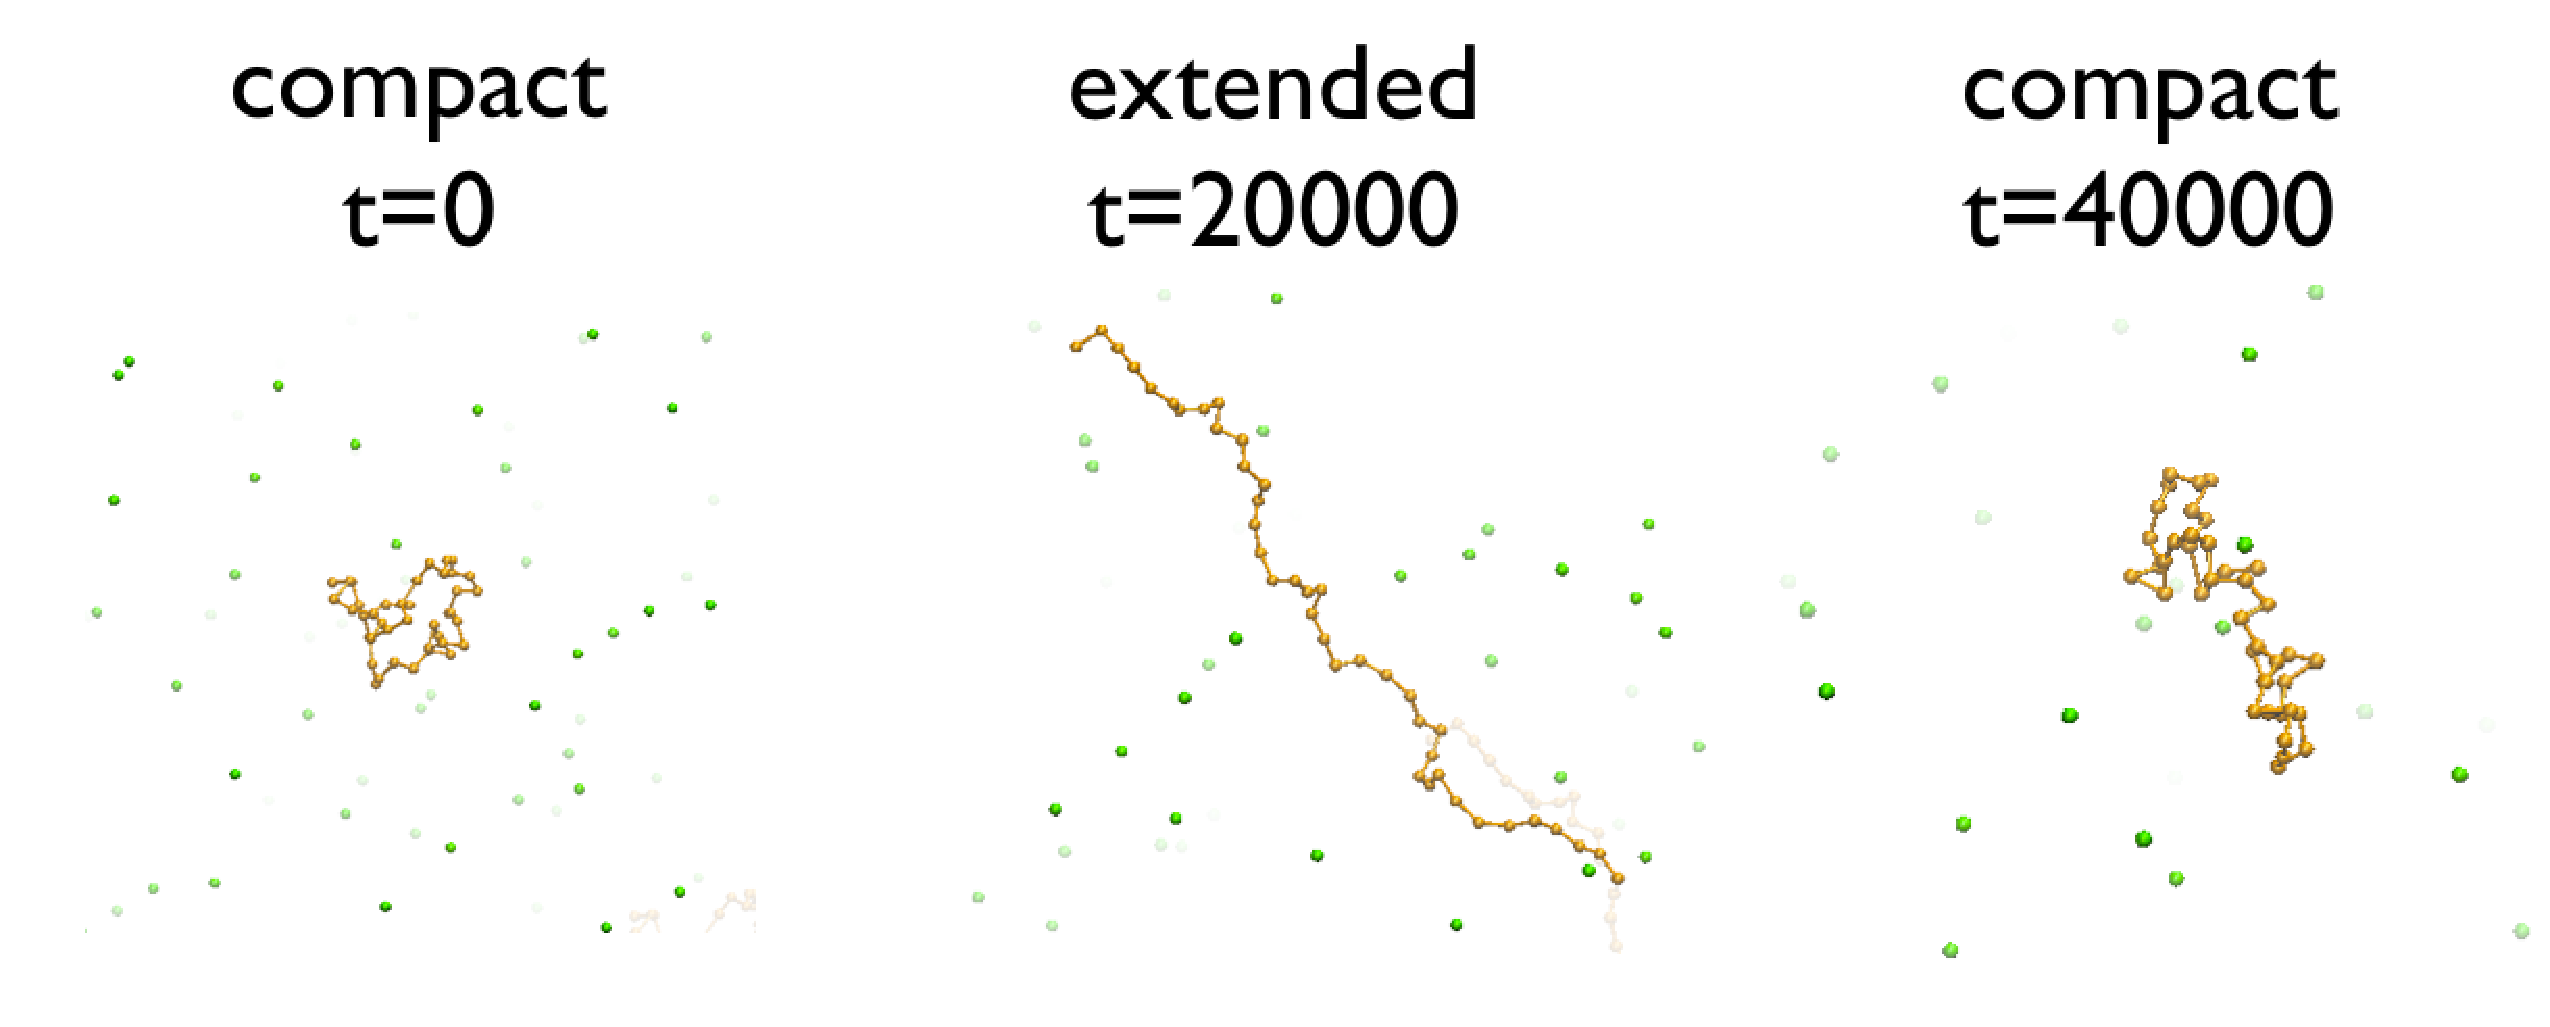
\includegraphics[width=15cm,angle=0]{./figures/compact-extended}
\caption{Simulation snapshots during the pulling forward and backward}
\label{picwork}
\end{center}
\end{figure} 

So with this example I hope that you can appreciate that you can let the system doing what you want to do with a limited amount of computational time. Nevertheless one should keep in mind that such times are generally shorter than the time that a standard MD would take to make a comparable displacement and, as such, they risk to be \uline{highly unrealistic}.
In normal conditions better to use slower steering speeds, which in general reduces the difference in work profile between  forward and backward or use different other techniques like metadynamics or umbrella sampling which will be introduced later.  

\section{An example with coordination number}
On top of this one might want to try other exotic experiment. For example, is it possible to then clusterize all the other particles around the chain?
One can use for example the coordination number which is defined as sum of sigmoids between two set of atoms $N_A$ and $N_B$
\begin{equation}
C({\bf x})=\sum_i^{N_A} \sum_j^{N_B}
\frac{1-\left(\frac{\vert{\bf x}_i - {\bf x}_j \vert}{r_0} \right)^{nn}}{
   1-\left(\frac{\vert{\bf x}_i - {\bf x}_j \vert}{r_0} \right)^{mm} }
\end{equation}
You can see again this function with \texttt{gnuplot}
by using the following commands
\begin{verbatim}
gnuplot> r0=3;nn=14;mm=16
gnuplot> f(x)=(1-(x/r0)**nn)/(1-(x/r0)**mm)
gnuplot> set xr [0:10]
gnuplot> plot f(x)
\end{verbatim}
In this example we used the exact values of $nn$, $mm$ and $r_0$ that we used in the example.
The plot of this function is shown in Fig. \ref{coordination}.
You can note that the coordination function is   rapidly decaying for value larger than 2.5 distance units and then, after 6, decays very slowly. Therefore, when all the atoms of the group $A$ are close to the atoms of group $B$ this will be a high number since all the sigmoids will provide a high number (close to 1). If the two set of particles are on average rather far from each other, then the coordination number will be low since the contribution of each sigmoid will be low.

\begin{figure}[h!]
\begin{center}
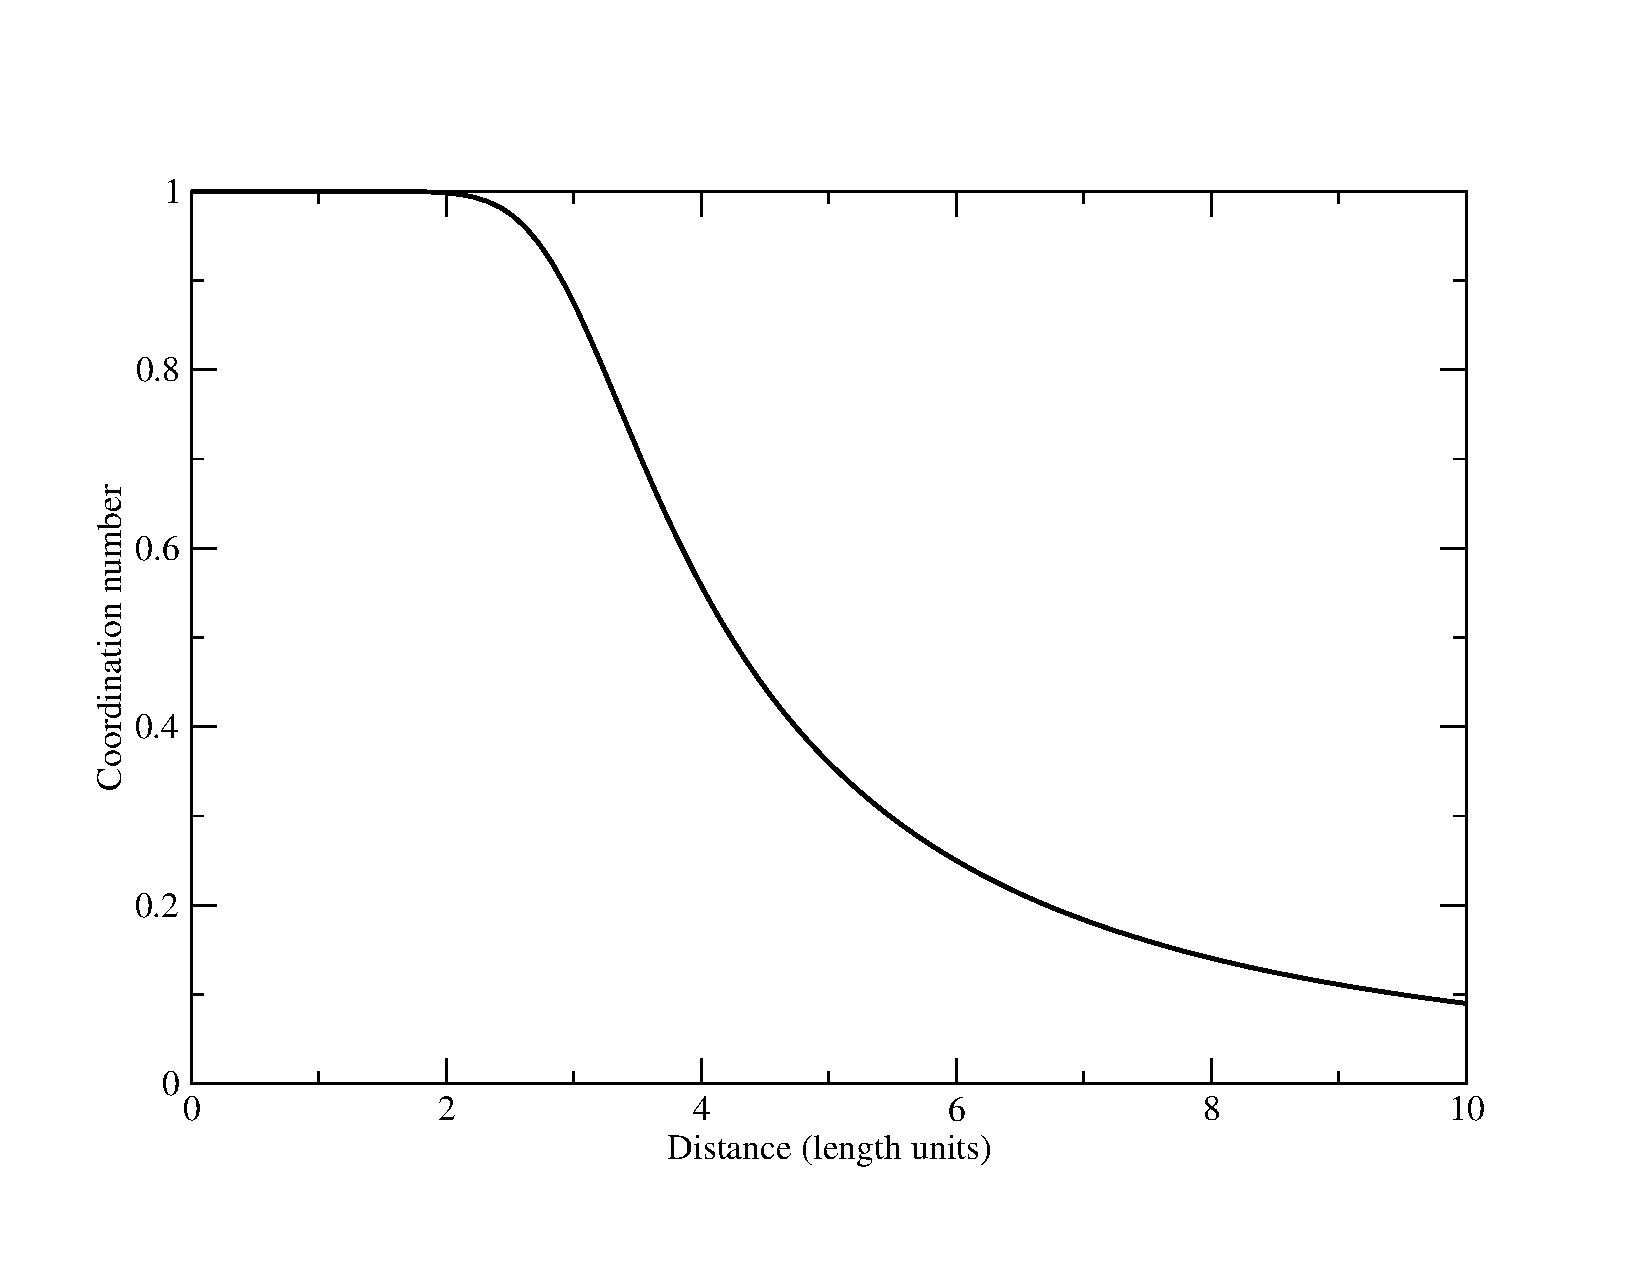
\includegraphics[width=12cm,angle=0]{./figures/coordination_plot}
\caption{Plot of the coordination number}
\label{coordination}
\end{center}
\end{figure} 

We can apply a force on this number and make so that is will artificially increase, similarly to what we have done for the end-to end distance. 
To this end we can hack the plumed input in this way

\begin{verbatim}
# a end-to-end distance
d1: DISTANCE ATOMS=1,40
# a coordination number of the other particles
c1: COORDINATION GROUPA=1-40 GROUPB=41-80 R_0=3.0 NN=14 MM=16
# a moving restraint using d1: note that the kappa is kept if not specified
MOVINGRESTRAINT ...
  ARG=d1
  STEP0=0      AT0=2.0   KAPPA0=5.0
  STEP1=20000  AT1=40.0
... MOVINGRESTRAINT
# another moving restraint after the steer
 MOVINGRESTRAINT ...
  ARG=c1 LABEL=sc1
  STEP0=20000  AT0=0.0   KAPPA0=0.0
  STEP1=40000  AT1=1200.0 KAPPA1=0.1
... MOVINGRESTRAINT
PRINT ARG=* STRIDE=50 FILE=COLVAR
PRINT ARG=c1,sc1.* STRIDE=50 FILE=COLVAR_COOR
\end{verbatim}
where you can see that we stretch the polymer along the distance for the first 20000 steps and then we proceed to steer the coordination number of the polymer with the particles as well.

What do you expect? Play the example and have a look with vmd. Is it what you expected? Why is so? (see Fig.  \ref{coord_traj})

\begin{figure}[h!]
\begin{center}
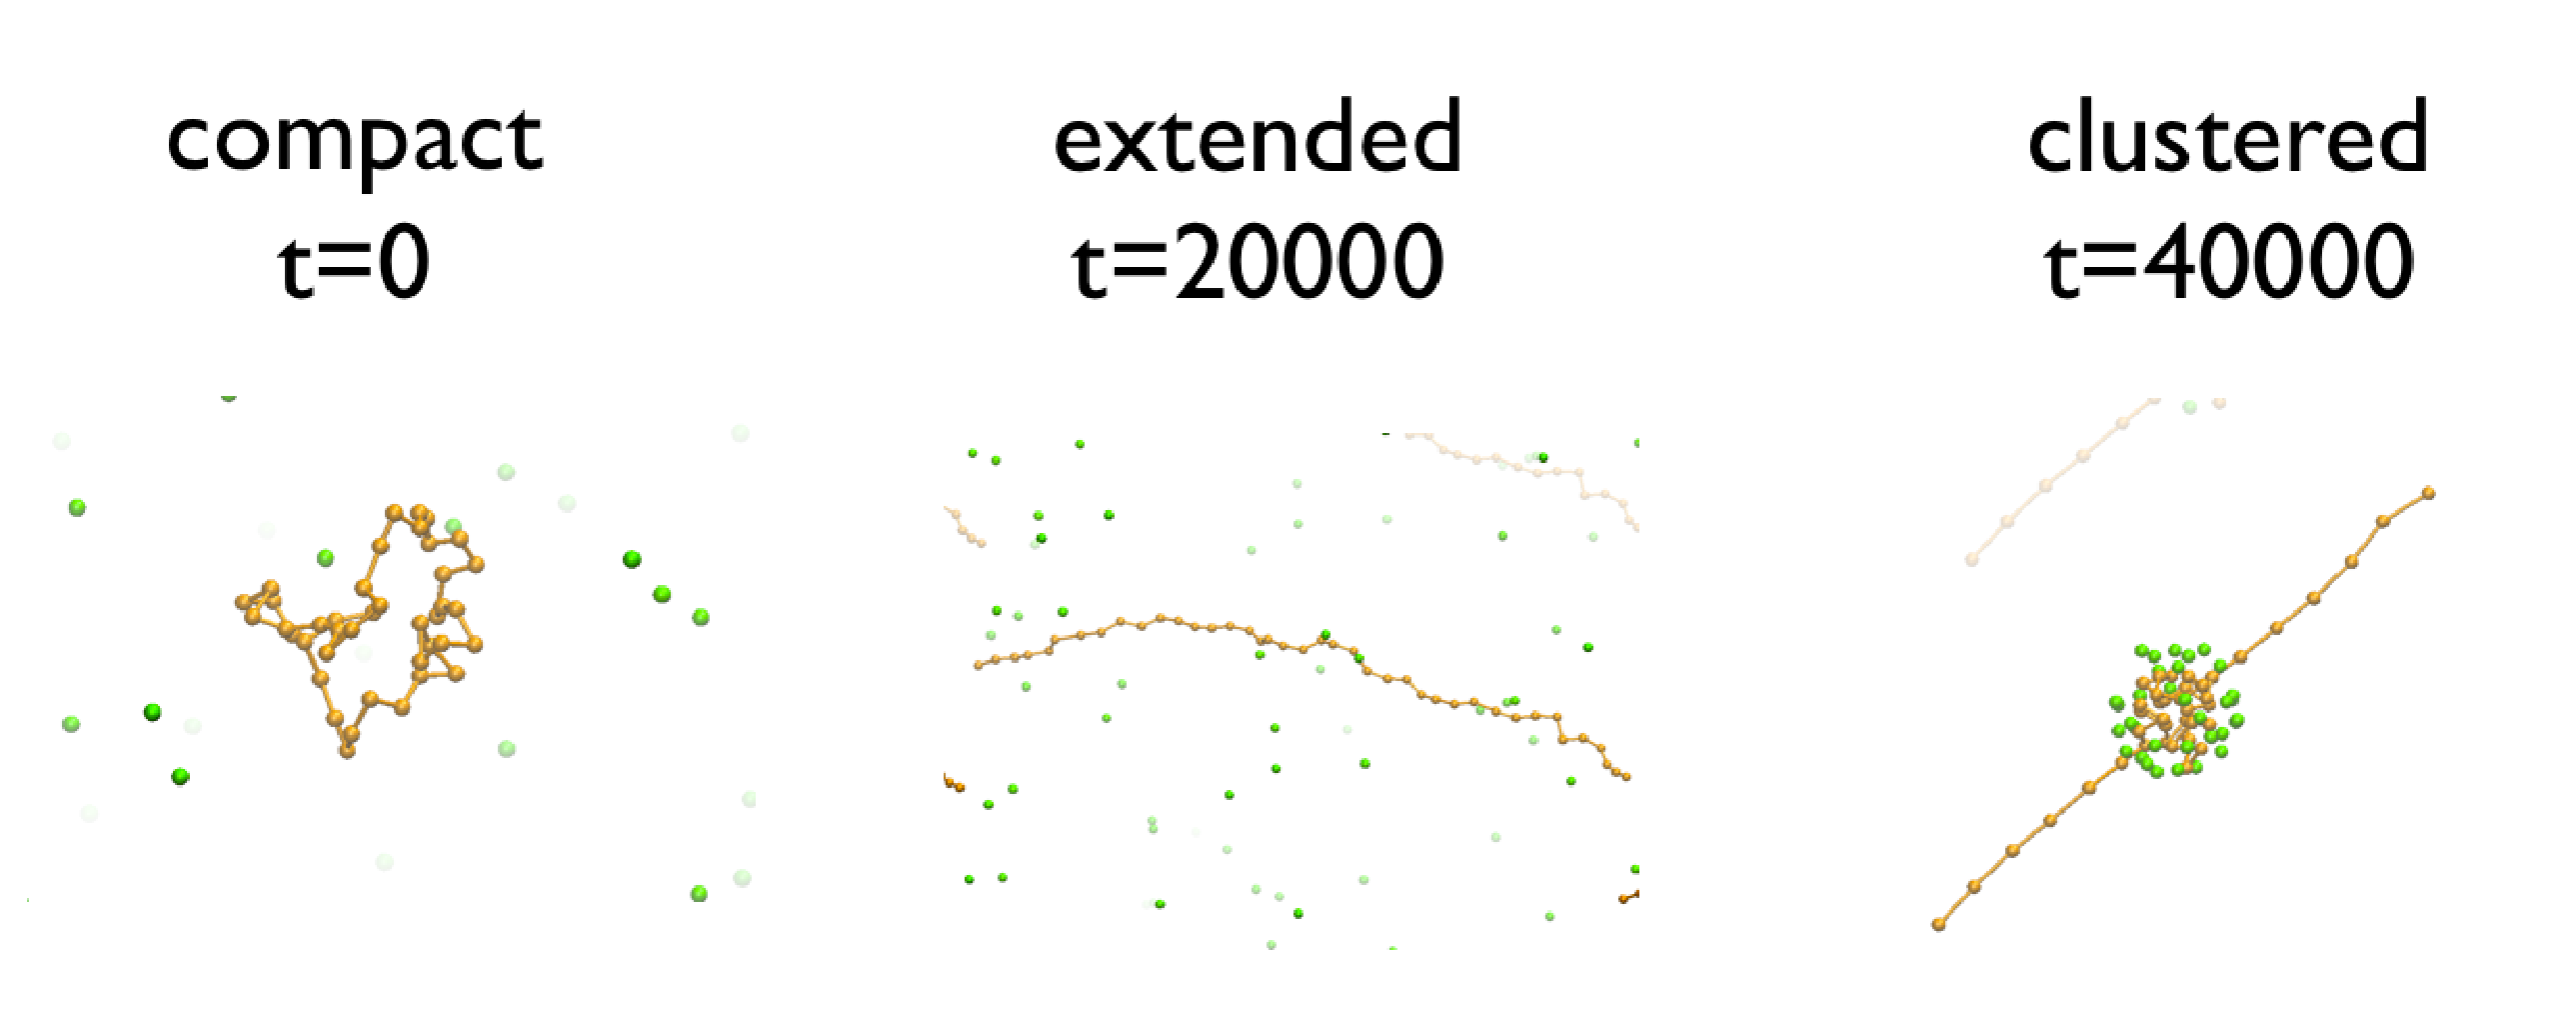
\includegraphics[width=15cm,angle=0]{./figures/coord_traj}
\caption{Plot of the coordination number}
\label{coord_traj}
\end{center}
\end{figure} 


One of the reasons why the particles cluster at the center of the polymer is that in that position, for each particle will have a lot of contributions from the chain, many more than if that was at the edges.

One could argue that in order to have something more realistic one should have a sharper cutoff so that the function decays rapidly within one single monomer length. Unfortunately in bias methods the long tails serve a vital role since the real force acting on the atoms is 
\begin{equation}
{\bf f}_i=-k(C({\bf x}) -c_0-vt)\frac{\partial C({\bf x}) }{\partial {\bf x}_i}
\end{equation}
therefore, even if the first term can be increased arbitrarily by using a larger
spring constant, the second washes away its effect if the coordination number is flat. 

This is an important observation that one should keep in mind when designing  biasing scheme.
The derivative of the collective coordinate which one is driving must be nonzero in the whole conformational domain that one intends to sample.

Note that so far this is just showing what is the power of accelerating the dynamics by using biasing forces. Note that the examples are all but physically relevant since the steering speeds adopted are not suitable for the system. In general a more gentle touch (smaller speed) should be able to recover a more realistic picture of the event.



\chapter{Biasing the system: metadynamics}

If you study a system for which you have either a barrier or a large free energy difference to move from one state to the other, like, in our example, from collapsed to extended state, 
it might well be that you never get to one of the two states, while starting from the other. 
Nevertheless we have seen that introduction of proper forces/biases may enhance the transition. 

Here we want to discuss the relation between free energy difference and an externally introduced bias.

Let's start from the common definition of Helmoltz free energy as function of a single order parameter.
\begin{eqnarray}
F(s_0)&=&-\frac{1}{\beta} \ln P(s_0)\\
 &=&-\frac{1}{\beta} \ln \frac{\int e^{-\beta V({\bf x})} \delta(s({\bf x})-s_0) d{\bf x}}{Q}
\end{eqnarray}
with $Q$ being the canonical partition function:
\begin{equation}
Q=\int e^{-\beta V({\bf x})}  d{\bf x} \ .
\end{equation}
Now we can relate this free energy with the one obtained from a biased ensemble in which we use 
a function $V_b(s)$ of some sort which bias the specific degree of freedom we're looking to. This would read
\begin{eqnarray}
F_b(s_0)&=&-\frac{1}{\beta} \ln P_b(s_0)\\
 &=&-\frac{1}{\beta} \ln \frac{\int e^{-\beta (V({\bf x})+V_b(s({\bf x})))} \delta(s({\bf x})-s_0) d{\bf x}}{Q_b}
\end{eqnarray}
with 
\begin{eqnarray}
Q_b=\int e^{-\beta (V({\bf x})+V_b(s({\bf x}))}  d{\bf x} 
\end{eqnarray}
Since all the points selected by the delta function $\delta(s({\bf x})-s_0)$ present the same value of $V_b(s({\bf x}))$, the exponential related to the bias can be pulled out from the integral to give:
 \begin{eqnarray}
F_b(s_0)&=&-\frac{1}{\beta} \ln e^{-\beta V_b(s_0)}\frac{\int e^{-\beta V({\bf x})} \delta(s({\bf x})-s_0) d{\bf x}}{Q_b}\\
&=&V_b(s_0)-\frac{1}{\beta} \ln \frac{\int e^{-\beta V({\bf x})} \delta(s({\bf x})-s_0) d{\bf x}}{Q_b}\\
&=&V_b(s_0)-\frac{1}{\beta} \ln P(s)\frac{Q}{Q_b}\\
&=&V_b(s_0)-\frac{1}{\beta} \ln P(s)+\frac{1}{\beta} \ln \frac{Q}{Q_b}\\
&=&V_b(s_0)-\frac{1}{\beta} \ln P(s)+C\\
F_b(s_0)&=&V_b(s_0)+F(s_0)+C
\end{eqnarray}
from which one has:
\begin{equation}
F(s_0)=F_b(s_0)-V_b(s_0)+C
\label{equnbias}
\end{equation}
that means that, from a biased simulation, one can retrieve the correct free energy just by knowing the bias and the histogram
in the biased ensemble. So, if one can find a function that compensates the free-energy landscape, then the system is free to travel in the space of CVs and the histogram can be acquired with accuracy since all the metastabilities are removed.
This is crucial for many enhanced sampling methods
and here we will discuss in particular Metadynamics (MetaD) \cite{metad} that relies exactly on an
iterative procedure aimed to produce the compensating potential.


Metadynamics adds an adaptive potential to the simulation that grows with simulation time.
Intuitively its functioning relies on Eq. \ref{equnbias} and, in order to find the best possible approximation to the perfectly compensating bias it adopts a history dependent potential. 
This bias potential acts on a restricted number of degrees of
freedom of the system $\bm{s}(x)=(s_1	(x),...,s_d(x))$ often referred to as collective variables or CVs.
The metadynamics potential $V(s,t)$ varies with time $t$ and is constructed 
as a sum of Gaussian functions, or hills, deposited during the simulation:

\begin{equation}
V(\bm{s},t)=\int_0^t\ dt^\prime \omega\exp\left(-\sum_{i=1}^{d} 
\frac{(s_i({\bf x})-S_i({\bf x}(t^\prime))^2}{2\sigma_i^2} \right),
\end{equation}

where $\sigma_i$ is the Gaussian width corresponding to the $i$-th CV
and $\omega$ the rate at which the bias grows.
In the practice, Gaussians of height equal to $W$ are deposited every $\tau$ MD steps,
so that $\omega=W / \tau$.

The function of these Gaussian potentials is to discourage the system to revisit the previously visited points in CV space and reach the point
in which all the points in CV space are equally sampled in time that delivers a flat histogram which has no contribution on the free energy. Under this assumption the Helmoltz free energy results to be  the negative of the deposited bias.

In order to perform a metadynamics simulation we have to:
\begin{itemize}
\item Choose wisely the set of CVs to address the problem. This is a long story. 
To cut it short, CVs 
a)  should clearly distinguish between the initial state, the final state and the intermediates,
b) should describe all the slow events that are relevant to the process of interest,
c) their number should not be too large, otherwise it will take a very long time to fill the free energy surface.
d) besides being good descriptors they should also be able to produce a force in a direction which is effectively enhancing the motion toward the transition state(s).

\item Choose the Gaussian height $W$ and the deposition stride $\tau$.
These two variables determine the rate of energy added to your simulation. 
If this is too large, the free-energy surface will be explored at a fast pace, 
but the reconstructed profile will be affected by large errors. 
If the rate is small, the reconstruction will be accurate, but it will take a longer time.
The error on the reconstructed FES depends on the ratio $W/\tau$, not on the two parameters alone \cite{error}.
\item Choose the Gaussian width $\sigma_i$. This parameter determines the resolution
of the reconstructed FES. The sum of Gaussians reproduces efficiently 
(\emph{i.e.} in a finite simulation time) features of the FES on a scale larger than $\sigma_i$. 
A practical rule is to choose the width as a fraction (half or one third) of the
CV fluctuations in an unbiased simulation. This is not a golden rule, since the value of the fluctuations
is not universal but usually depends on the position in the CV space (see Fig. \ref{fluctuation} for the calculation 
of the fluctuation on the CVs used for tracking the unbiased dynamics). 
In particular, although intuitively a larger $\sigma$ could bring to a faster filling, very often, when the choice is not clear as in \ref{fluctuation} it is much better to adopt the smaller one since it guarantees a better resolution and ability to fill up both narrow and large wells.
\end{itemize}

In this exercise one first needs to have a look to the output file \texttt{COLVAR} of our first exercise. By plotting the timeline
\begin{verbatim}
gnuplot> plot "COLVAR" u 1:2
\end{verbatim}
one immediately realises that the fluctuations are around 50 time steps and cover around 4 units in distance. There are also larger breathing motions up 20 distance units but here we try to exploit those small fluctuation. So, assuming that those values are identical in all the distance domain, we will use a time interval for Gaussian deposition of 100 time step and a $\sigma$ of 4.  
Note that using excessively small sigma, although intuitively should pose no problem since the energy which is introduced is very small, as a matter of fact it results in a set of very steep hills (which depend on the highest value of Gaussian derivative) whose forces can screw up the integrator! On the contrary too large hills do not result in a faster filling but in a small force (the maximum derivative of the Gaussian becomes small), which drives the system in a slower way.  

Since the temperature is set to 1 we adopt hills which are a fraction of it, say 0.3.

The input file for metadynamics actually has only one line more 
\begin{verbatim}
# the usual distance
d1: DISTANCE ATOMS=1,40
# metadynamics on the distance labelled with d1
# 0.3 hills height every 100 
meta: METAD  ARG=d1 SIGMA=4.0 HEIGHT=0.3 PACE=100
PRINT ARG=* STRIDE=50 FILE=COLVAR
\end{verbatim}

By default this input generates an additional file called \texttt{HILLS}
which formatted like this
\begin{verbatim}
#! FIELDS time d1 sigma_d1 height biasf
#! SET multivariate false
            1      2.551184033653086           4        0.3        1
            2      2.291870216662208           4        0.3        1
            3      2.784452843494628           4        0.3        1
            ...
\end{verbatim}
where, as reported in the header, includes the time, the point in phase space where the
Gaussian is deposited, the width, the height and a bias factor (only useful when using Well-tempered metadynamics). The flag \texttt{multivariate} sets off the use of adaptive Gaussians
which introduce variable shape and size hills.

The file \texttt{HILLS} needs the plumed executable to be processed.
The command
\begin{verbatim}
 plumed sum_hills --stride 300 --hills HILLS
\end{verbatim}
post processes the file \texttt{HILLS} and produce the free energy estimate produced from the bias every 300 deposited Gaussian potentials. 

Ideally, after having flattened the free energy, one should retrieve a free energy profile which is the same at every iteration, except for a constant.

By plotting the free energies with gnuplot
\begin{verbatim}
gnuplot> plot "fes_0.dat" w l, "fes_1.dat" w l, "fes_2.dat" w l
gnuplot> repl "fes_3.dat" w l, "fes_4.dat" w l
\end{verbatim}
one can get something like the graph reported in Fig. \ref{free_ene}

\begin{figure}[h!]
\begin{center}
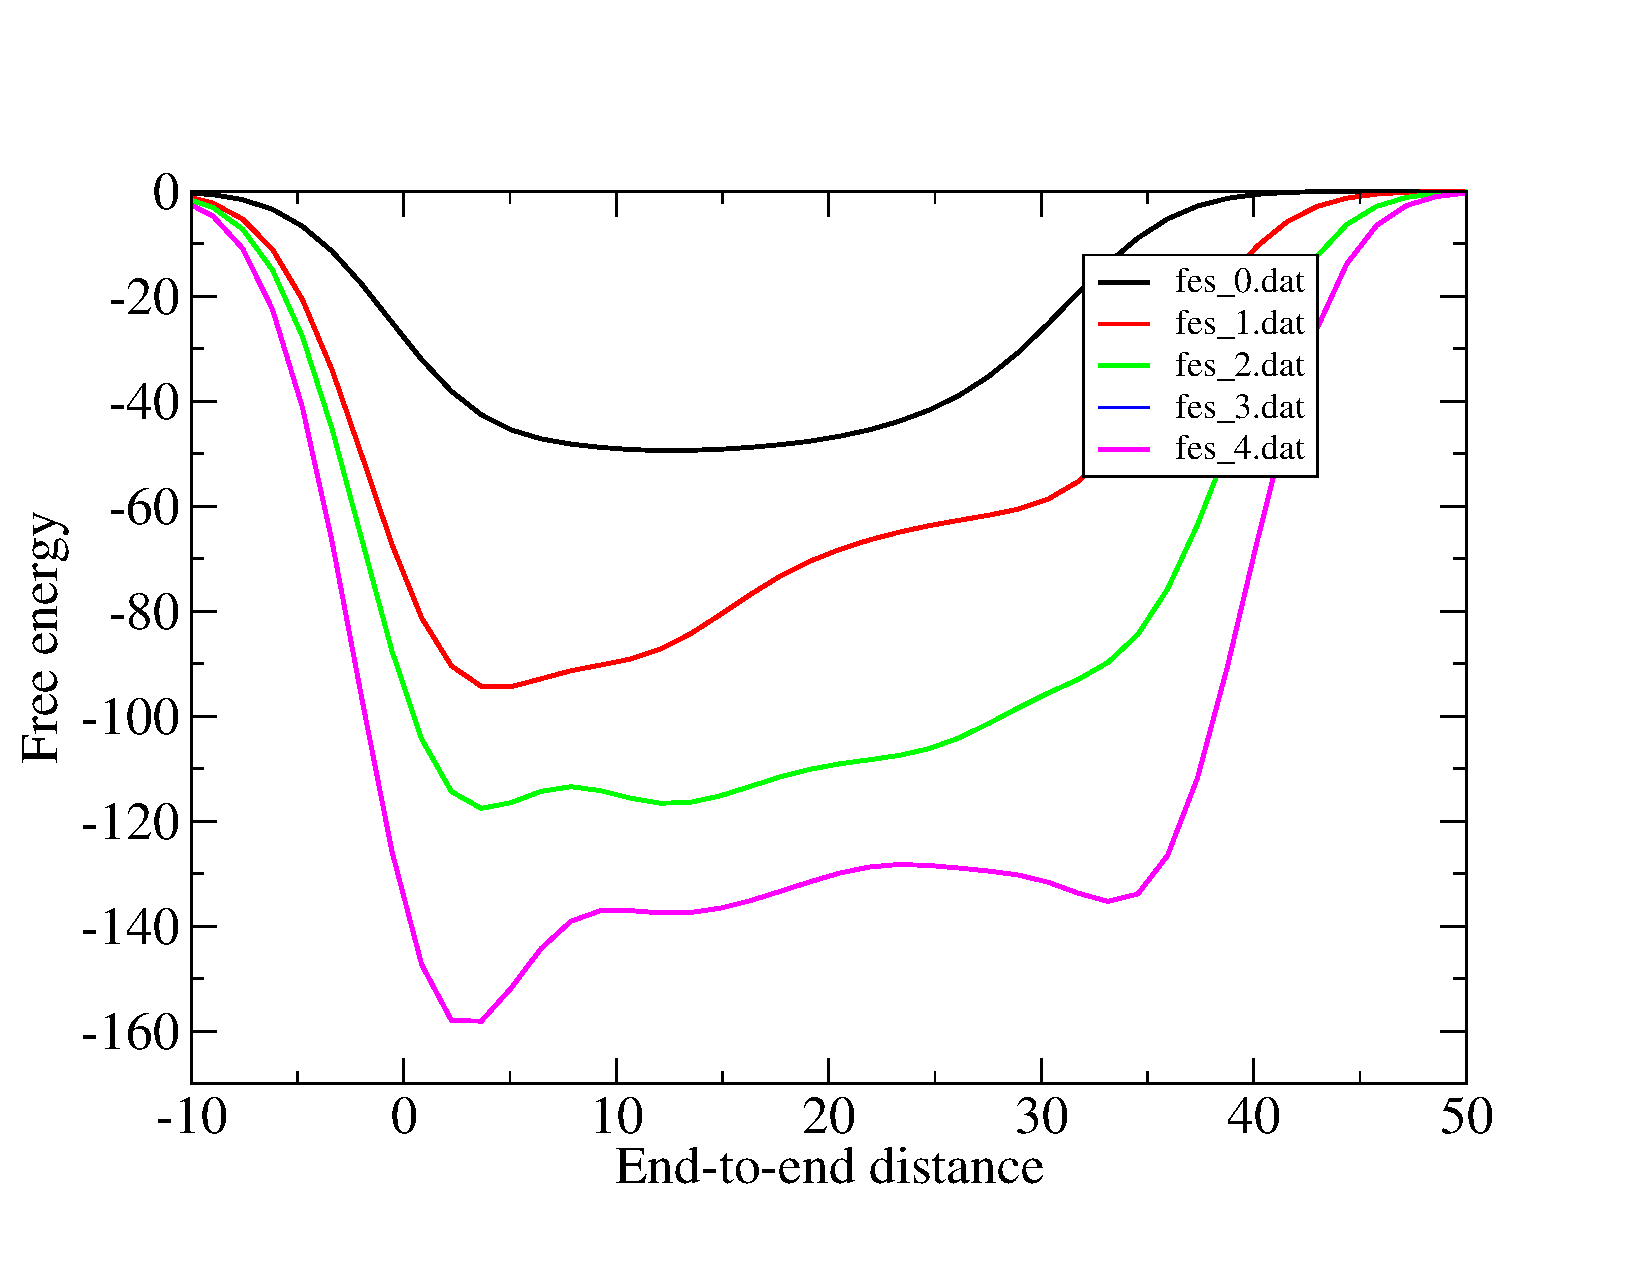
\includegraphics[width=15cm,angle=0]{./figures/free_energy}
\caption{Plot of the free energy as function of the end-to-end distance as obtained by metadynamics}
\label{free_ene}
\end{center}
\end{figure} 

There are various interesting features of this plot
\begin{itemize}
\item The free energy seems to span also on negative values of end-to-end distance. Is it wrong? No, it is just that the Gaussian deposited by metadynamics does not know that the distance cannot be negative and when a Gaussian is deposited, say, at two units of distance, then it is likely to span to values less than zero. Keep it in mind: larger hills mean coarser representation.
The same is true for large values: your system hardly spans distance larger than 35 distance units, nevertheless the accumulation  of the tail of the  Gaussian potential may give you the fake impression that you are sampling values beyond that value. Just make up your mind plotting the second column in \texttt{HILLS} file.
\item the free energy doesn't evenly grow along the profile. This generally point to two possible problems: either the potential is grown too fast (and \texttt{HEIGHT} should decrease or \texttt{PACE} should be increased) or the descriptor is not right for the problem under study
\item the minimum is not well defined. While in the first profile the minimum is in the center, in the others the minimum is in a compact state and finally in the last both compact and extended states are metastable. When this happens at the extreme conformations one should have a look at the sigmas, just to check if, when the simulation is at one of the endpoints the fluctuations are comparable respect to the sigma of the hills. If not, then the system substantially see a flat potential (sum of large hills) that does not impose a repulsive force.
\end{itemize}

In order to better understand and solve this last point lets have a look to the timeline of the 
\texttt{HILLS} file.

\begin{verbatim}
gnuplot> p "HILLS" u 1:2:3 w yer,"" u 1:2 w lp
\end{verbatim}

\begin{figure}[h!]
\begin{center}
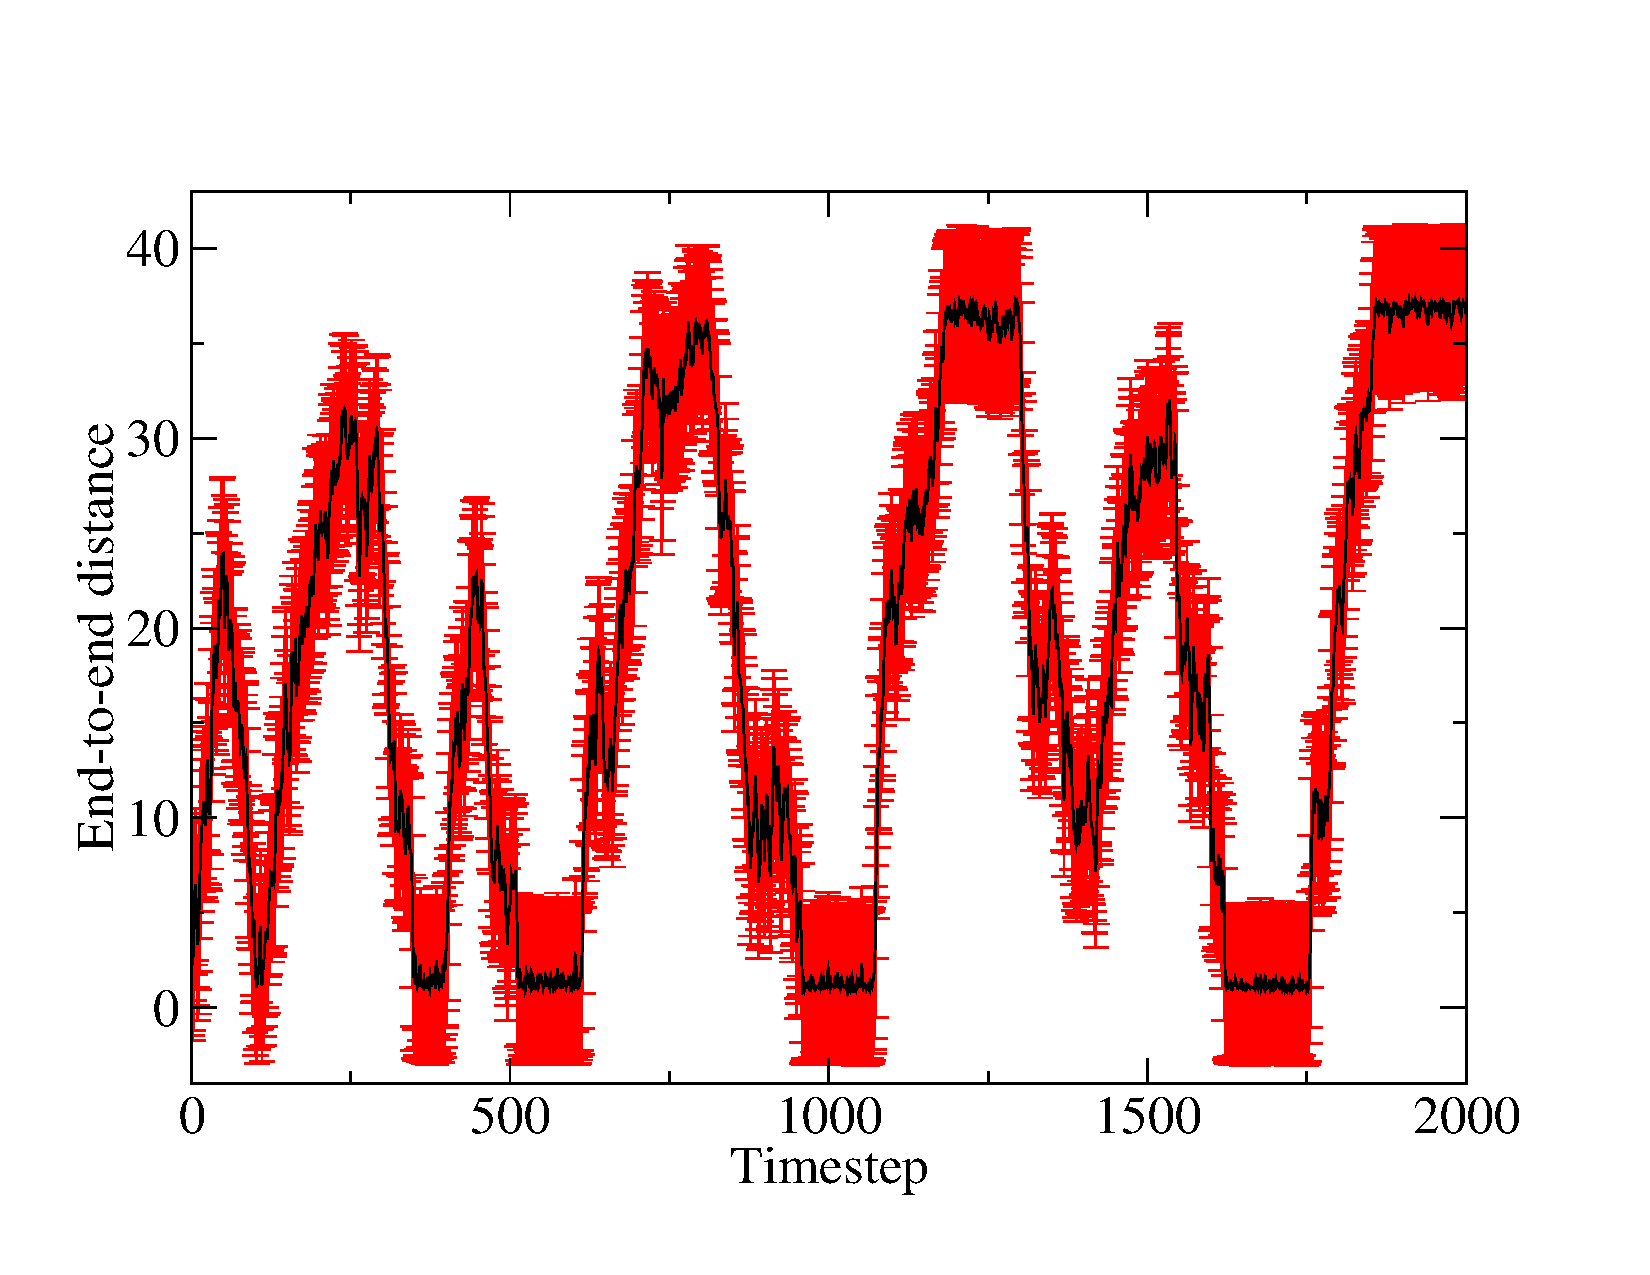
\includegraphics[width=15cm,angle=0]{./figures/timeline}
\caption{Plot of the time evolution of hills along with their respective width. It is evident that at the edges the hills are over accumulated and the system is stuck.}
\label{timeline}
\end{center}
\end{figure} 

Hey, you really see that the system bounces back and forth. This is what you want since this is allowing you to explore faster the conformational space. What you do not want is that it stops for such png time at the boundaries (see end-to-end distances around 2 and 25 distance units) since, when metadynamics is filling the potential energy landscape there is no reason for the system to stop there. Just observe what is happening there: the system just have tiny fluctuation at the boundaries and if you accumulate large hills but you are on top of them, the force that your system experiences is zero since, at the top of a very large mountain, the gradient is zero. This dictates the hills width that one has to use, in this case I would retry with hills of 1.0 sigma.

Another important observation comes from the fact that hills seem to overlap with each others, even when they move fastly from one region to the other. This points to the fact that there might be some effect of the system "surfing" on the hills, so, instead of compensating the underlying free energy landscape, metadynamics is actually creating "waves" of bias that do not converge.

This can be resolved with a reduced deposition rate (i.e. \texttt{PACE}), for example 400 timesteps. This means also that the free energy landscape will be filled more slowly so it will be need to increase the simulation time as well. This can be done in the usual way in the ESPResSo script (say twice as big). 

The resulting time evolution is shown in Fig. \ref{timeline2} which is typical of a reasonable metadynamics evolution. Despite the larger simulation time, it is possible to appreciate that the span of the end-to-end distance is smaller respect to the other case but the hills are more scattered and not clustered at the extrema of the domain.

\begin{figure}[h!]
\begin{center}
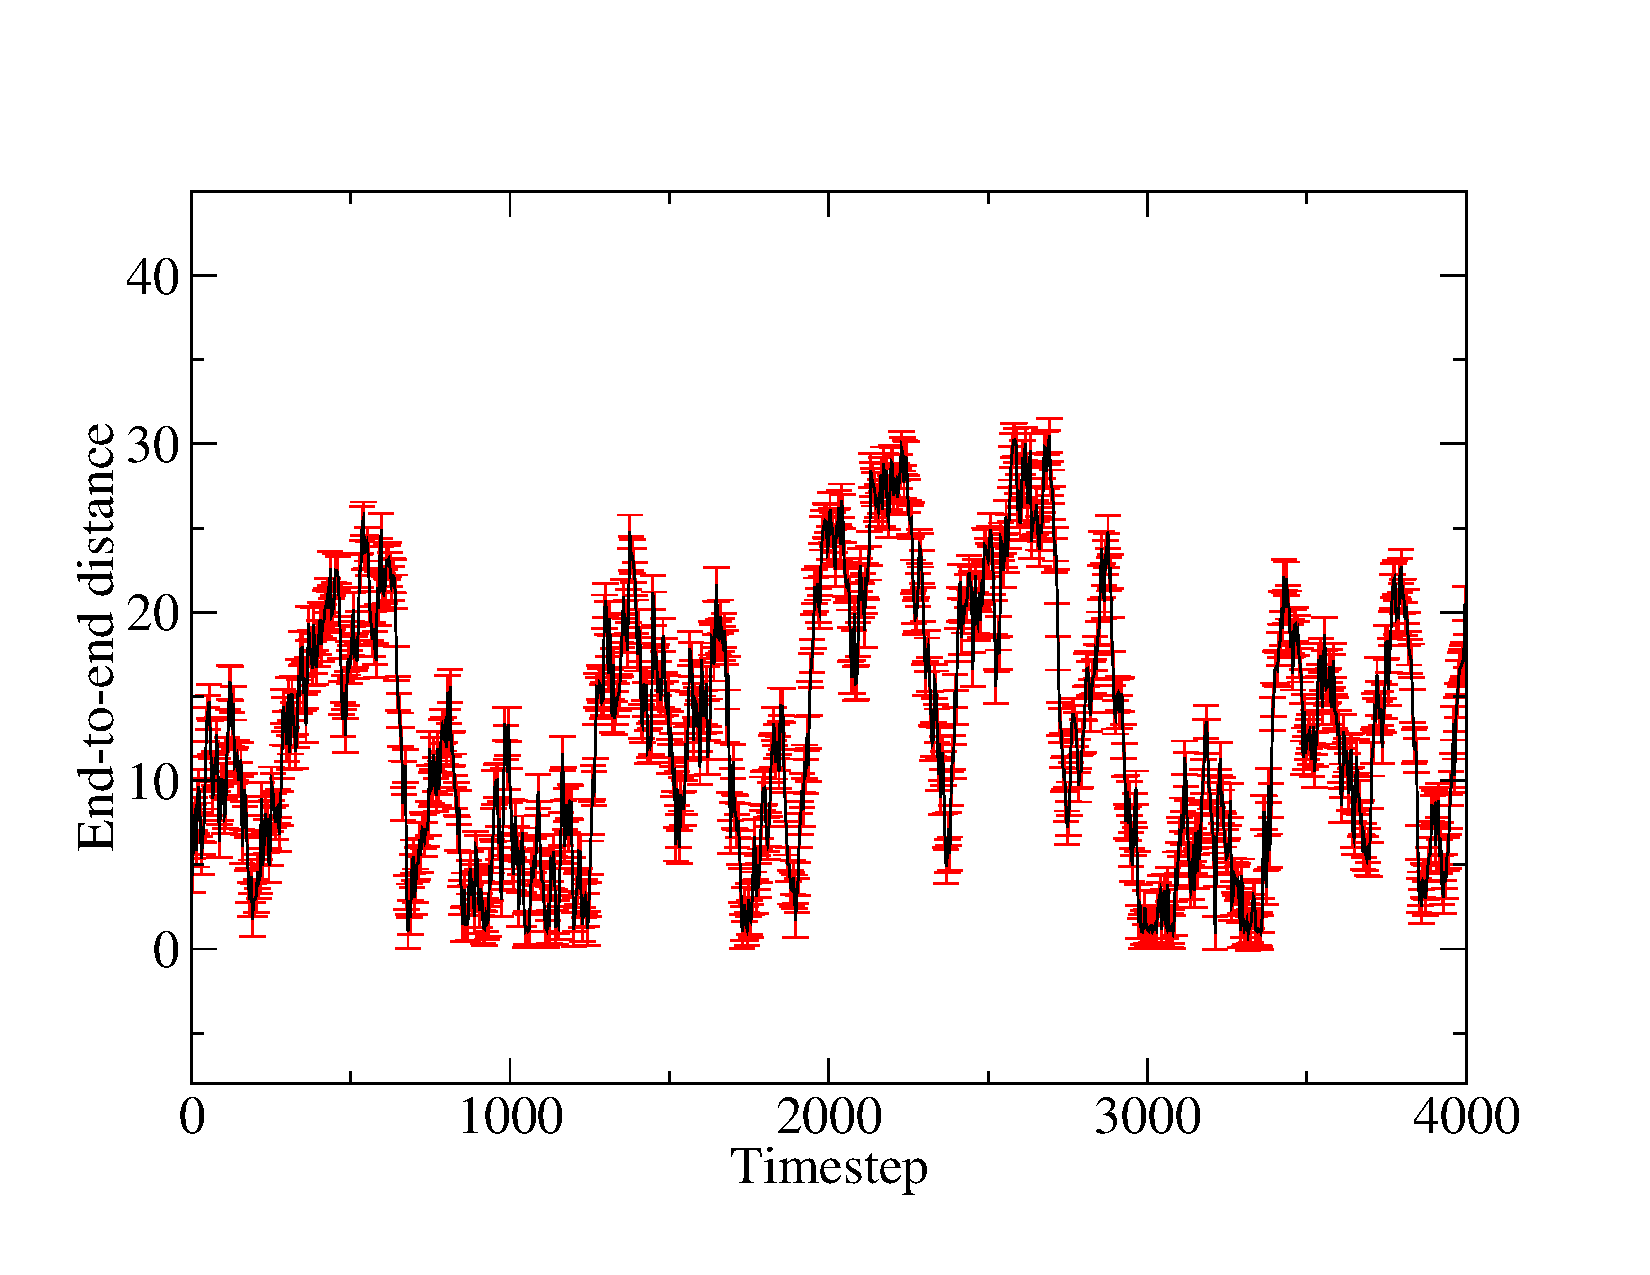
\includegraphics[width=15cm,angle=0]{./figures/timeline2}
\caption{Plot of the time evolution of hills along with their respective width for a reduced sigma and increased deposition time. The system is not stuck anymore.}
\label{timeline2}
\end{center}
\end{figure} 

The free energy profiles can be obtained through the following command

\begin{verbatim}
plumed sum_hills --stride 200 --hills HILLS
\end{verbatim}

and, by plotting, one should obtain the profiles as in Fig. \ref{free_ene2}

\begin{figure}[h!]
\begin{center}
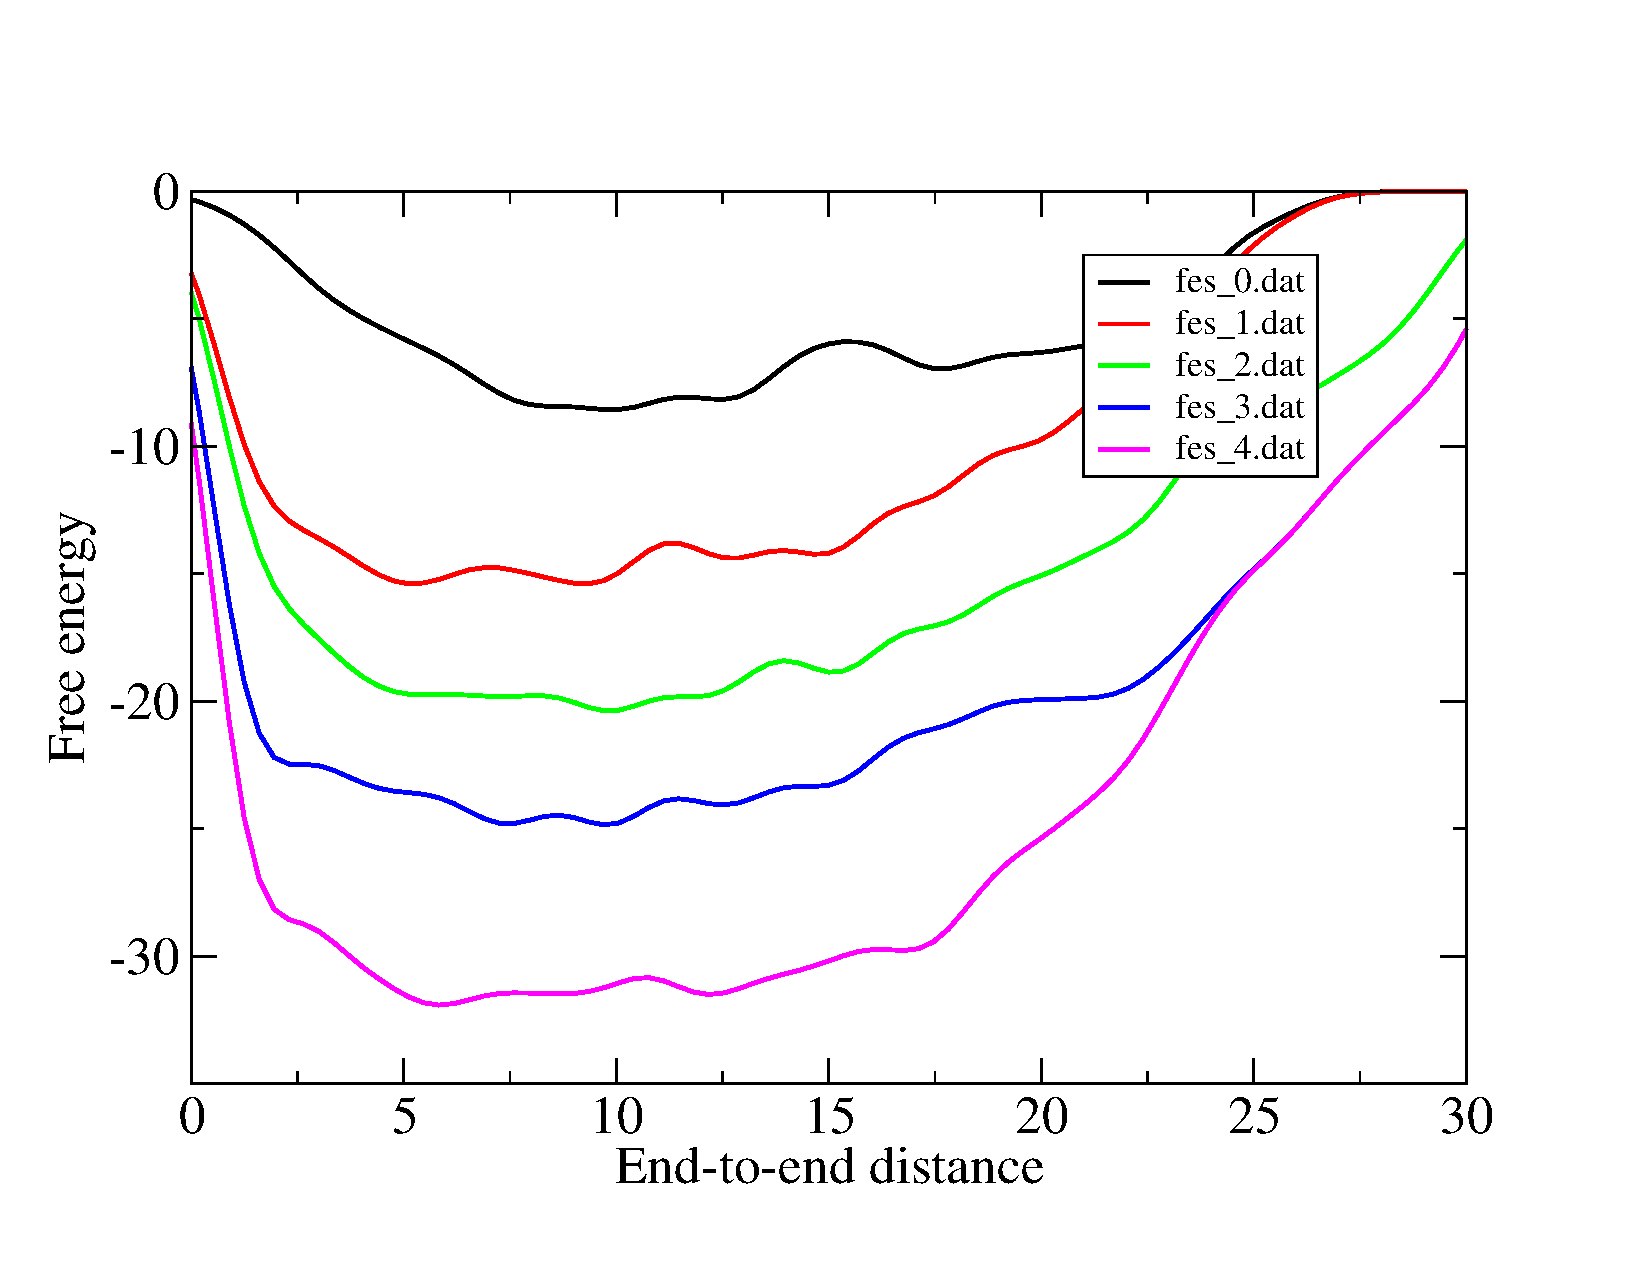
\includegraphics[width=15cm,angle=0]{./figures/free_energy2}
\caption{Plot of the free energy as function of the end-to-end distance as obtained by metadynamics with a smaller width and larger deposition rate.}
\label{free_ene2}
\end{center}
\end{figure} 

It is possible to appreciate that in this case the free energy profiles grow more parallel to each other in the most sampled region (i.e. from 2 to 20 in end-to-end distance) which is a sign of good choice  of parameters. 

If one wants to further reduce the difference between a free energy estimate and the next then the problem that needs to be faced is using a different collective variable. End to end distance can be a very rough order parameter indeed. Using contact maps or gyration radius can be some valid alternatives. In case of protein folding one could also consider something that reproduce a specific order in the  formation of contacts. PLUMED2.0 provides a large set of these.


\chapter{Where do I go from here?}
These small set of exercises cover just a small set of the capabilities of PLUMED2.0. 
Anyway, I recommend, before embarking any serious project based on enhanced sampling calculation, to devote time to read the literature and in particular the classic books
\cite{ALLE87,frenkelsmit,chandler} to acquire a solid background in both simulation techniques and statistical mechanics.

In this way you will also come to know other techniques included in PLUMED that, for the sake of 
conciseness, were not treated here. Among all it is worth citing
Umbrella Sampling \cite{torrie-valleau,wham1,wham2} and also various other
flavours of metadynamics such as
 multiple walkers metadynamics \cite{multiplewalkers}, well-tempered metadynamics \cite{Barducci:2008}, well-tempered ensemble\cite{Bonomi:2009p17935} and adaptive Gaussians
 \cite{Branduardi:2012dl}  to name a few that are implemented and ready to use together with ESPResSo  More than this, PLUMED2.0 allows to have plenty of CVs available: from angles to torsion to coordination number up to path collective variables \cite{brand07}. The investigation of the optimal space for projection of the free energy is a very active field indeed. In order to favour this, one can also build a personal collective variable through the \texttt{MATHEVAL} (requires \texttt{libmatheval} installed) without encoding the analytical derivatives which are automatically calculated by the library. You are encouraged to explore its capabilities through the online manual \url{http://plumed.github.io/doc-v2.0/user-doc/html/index.html}.

Additionally PLUMED2.0 can be used as a post processing tool, (try this command: \texttt{plumed driver --help}) and can be used to analyse output trajectories with PLUMED2.0 collective variables.

\bibliographystyle{./elsarticle-num}
%\phantomsection
%\addcontentsline{toc}{chapter}{Bibliography}
\bibliography{bibliography}
\printindex
%\newpage
%\thispagestyle{empty}
\mbox{}
\newpage
\end{document}
